\label{ssub:实验心得}
本次实验花费了7小时45分钟在C++排序程序代码编写上, 43分钟在makefile
用法的学习和编写上, 1小时57分钟在tex实验报告的编写上.\par
\begin{figure}[ht!]
	\begin{center}
		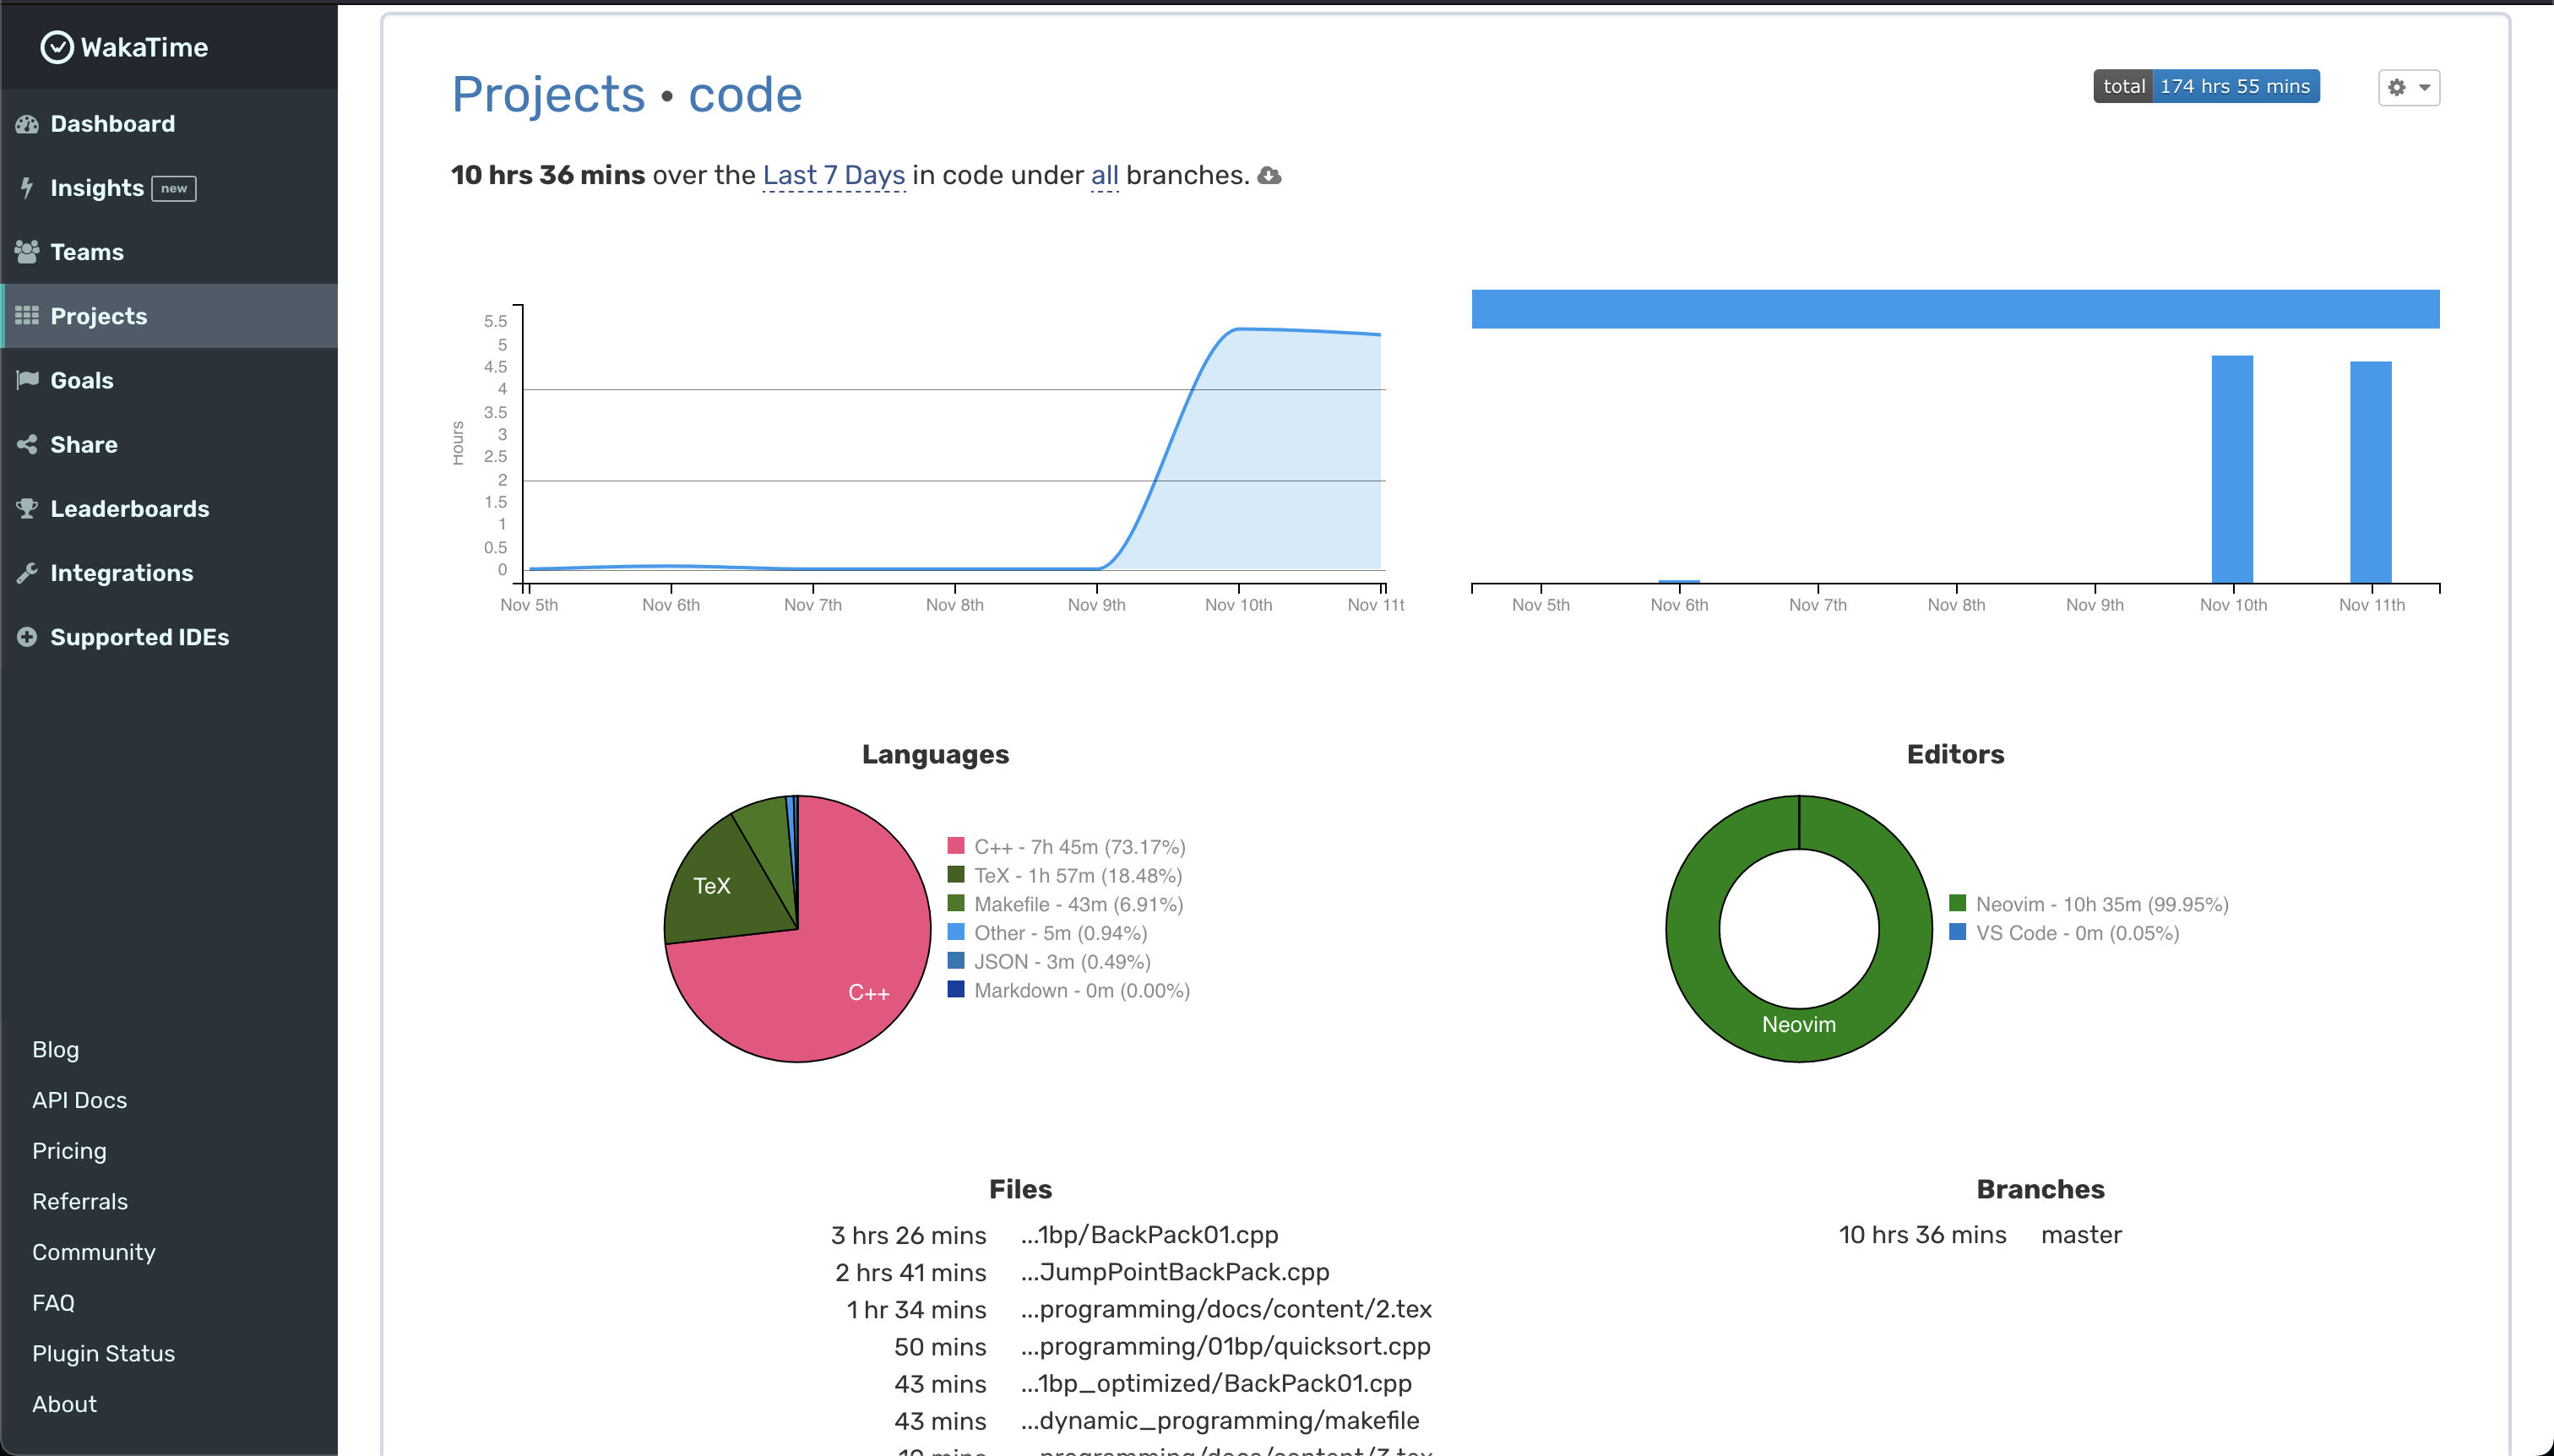
\includegraphics[width=0.95\textwidth]{figures/screenTime.png}
	\end{center}
	\caption{编写时间统计}
	\label{fig:screenTime}
\end{figure}


通过这次实验, 我动手实现了0-1背包问题的动态规划和跳跃点优化算法. 动手实践了
各算法的时间复杂度和空间复杂度分析. 此外, 为了综合评价各算法的
正确性, 以及衡量各算法的性能, 还动手实现了数据生成器, 用来
方便的生成指定数量的均匀分布在给定范围的随机排序的数据作为排序程序的输入.\par

在构建和管理项目的工具方面, 学习并使用了make工具, 方便的实现了
对程序的构建和测试; 此外, 对于文档, 也使用了make工具作为管理,
很大程度上方便了实验报告修改后的再次编译. 在实验报告编写方面,
练习了latex的使用, 对latex语法和使用更加熟悉.\par

但是, 由于时间有限, 没有实现更多的优化内容, 比如使用滚动数组压缩空间,
使用滚动数组优化跳跃点方法避免输入数据过多的时候占用空间指数级上升.\par

总的来说, 这次实验在动态规划算法之内及之外都学到了许多知识, 收获颇丰.
% subsection 实验心得 (end)
